\documentclass[]{article}
\usepackage[T1]{fontenc}
\usepackage{lmodern}
\usepackage{amssymb,amsmath}
\usepackage{ifxetex,ifluatex}
\usepackage{fixltx2e} % provides \textsubscript
% Set line spacing
% use upquote if available, for straight quotes in verbatim environments
\IfFileExists{upquote.sty}{\usepackage{upquote}}{}
\ifnum 0\ifxetex 1\fi\ifluatex 1\fi=0 % if pdftex
  \usepackage[utf8]{inputenc}
\else % if luatex or xelatex
  \ifxetex
    \usepackage{mathspec}
    \usepackage{xltxtra,xunicode}
  \else
    \usepackage{fontspec}
  \fi
  \defaultfontfeatures{Mapping=tex-text,Scale=MatchLowercase}
  \newcommand{\euro}{€}
\fi
% use microtype if available
\IfFileExists{microtype.sty}{\usepackage{microtype}}{}
\usepackage[margin=1in]{geometry}
\usepackage{longtable,booktabs}
\usepackage{graphicx}
% Redefine \includegraphics so that, unless explicit options are
% given, the image width will not exceed the width of the page.
% Images get their normal width if they fit onto the page, but
% are scaled down if they would overflow the margins.
\makeatletter
\def\ScaleIfNeeded{%
  \ifdim\Gin@nat@width>\linewidth
    \linewidth
  \else
    \Gin@nat@width
  \fi
}
\makeatother
\let\Oldincludegraphics\includegraphics
{%
 \catcode`\@=11\relax%
 \gdef\includegraphics{\@ifnextchar[{\Oldincludegraphics}{\Oldincludegraphics[width=\ScaleIfNeeded]}}%
}%
\ifxetex
  \usepackage[setpagesize=false, % page size defined by xetex
              unicode=false, % unicode breaks when used with xetex
              xetex]{hyperref}
\else
  \usepackage[unicode=true]{hyperref}
\fi
\hypersetup{breaklinks=true,
            bookmarks=true,
            pdfauthor={Heather E. Wheeler, Hae Kyung Im},
            pdftitle={Genetic Architecture of Transcriptome Regulation},
            colorlinks=true,
            citecolor=blue,
            urlcolor=blue,
            linkcolor=magenta,
            pdfborder={0 0 0}}
\urlstyle{same}  % don't use monospace font for urls
\setlength{\parindent}{0pt}
\setlength{\parskip}{6pt plus 2pt minus 1pt}
\setlength{\emergencystretch}{3em}  % prevent overfull lines
\setcounter{secnumdepth}{5}

%%% Change title format to be more compact
\usepackage{titling}
\setlength{\droptitle}{-2em}
  \title{Genetic Architecture of Transcriptome Regulation}
  \pretitle{\vspace{\droptitle}\centering\huge}
  \posttitle{\par}
  \author{Heather E. Wheeler, Hae Kyung Im}
  \preauthor{\centering\large\emph}
  \postauthor{\par}
  \predate{\centering\large\emph}
  \postdate{\par}
  \date{2015-04-30 12:41:51}




\begin{document}

\maketitle


\section{Abstract}\label{abstract}

\emph{Lorem ipsum dolor sit amet, est ad doctus eligendi scriptorem. Mel
erat falli ut. Feugiat legendos adipisci vix at, usu at laoreet
argumentum suscipiantur. An eos adhuc aliquip scriptorem, te adhuc dolor
liberavisse sea. Ponderum vivendum te nec, id agam brute disputando
mei.}

\section{Introduction}\label{introduction}

Lorem ipsum dolor sit amet, est ad doctus eligendi scriptorem. Mel erat
falli ut. Feugiat legendos adipisci vix at, usu at laoreet argumentum
suscipiantur. An eos adhuc aliquip scriptorem, te adhuc dolor
liberavisse sea. Ponderum vivendum te nec, id agam brute disputando mei.

Putant numquam tacimates at eum. Aliquip torquatos ex vis, mei et quando
debitis appareat, impetus accumsan corrumpit in usu. Nam mucius facilis
singulis id, duo ei autem imperdiet instructior. Cu ceteros alienum mel,
id vix putant impedit, ex idque eruditi forensibus eum. Posse dicunt id
usu. Ei iracundia constituto sed, duo ne exerci ignota, an eum unum
conceptam.

Has audire salutandi no, ut eam dicat libris dicunt. Pri hendrerit
quaerendum adversarium ea, dicat atqui munere et sea. Illum insolens eos
ne, eu enim graece rationibus mea. At postea utamur mel, eius nonumes
percipitur at vis. Numquam similique in per, te quo saepe utroque
pericula.

Ea nonumy volumus usu, no mel inermis dissentias. Dico partiendo
vituperatoribus eum et. Mea accusam convenire te, usu populo qualisque
gloriatur ut. Eu eum oratio altera option, ad mea ignota scriptorem. Ne
suas latine vix, eos oblique sanctus pertinax cu.

\section{Methods}\label{methods}

Lorem ipsum dolor sit amet, est ad doctus eligendi scriptorem. Mel erat
falli ut. Feugiat legendos adipisci vix at, usu at laoreet argumentum
suscipiantur. An eos adhuc aliquip scriptorem, te adhuc dolor
liberavisse sea. Ponderum vivendum te nec, id agam brute disputando mei.

Putant numquam tacimates at eum. Aliquip torquatos ex vis, mei et quando
debitis appareat, impetus accumsan corrumpit in usu. Nam mucius facilis
singulis id, duo ei autem imperdiet instructior. Cu ceteros alienum mel,
id vix putant impedit, ex idque eruditi forensibus eum. Posse dicunt id
usu. Ei iracundia constituto sed, duo ne exerci ignota, an eum unum
conceptam.

\subsection{Equations}\label{equations}

The deterministic part of the model is defined by this \textbf{in-line
equation} as $\mu_i = \beta_0 + \beta_1x$, and the stochastic part by
the \textbf{centered equation}:

\[ \frac{1}{\sqrt{2\pi}\sigma}e^{-(x-\mu_i)^2/(2\sigma^2)} \]

\subsection{Tables}\label{tables}

\begin{longtable}[c]{@{}lrrrr@{}}
\toprule\addlinespace
& Estimate & Std. Error & t value &
Pr(\textgreater{}\textbar{}t\textbar{})
\\\addlinespace
\midrule\endhead
(Intercept) & -0.08 & 0.09 & -0.94 & 0.35
\\\addlinespace
x & 1.86 & 0.10 & 19.51 & 0.00
\\\addlinespace
\bottomrule
\addlinespace
\caption{This is a GLM summary table.}
\end{longtable}

\subsection{Plots}\label{plots}

\begin{figure}[htbp]
\centering
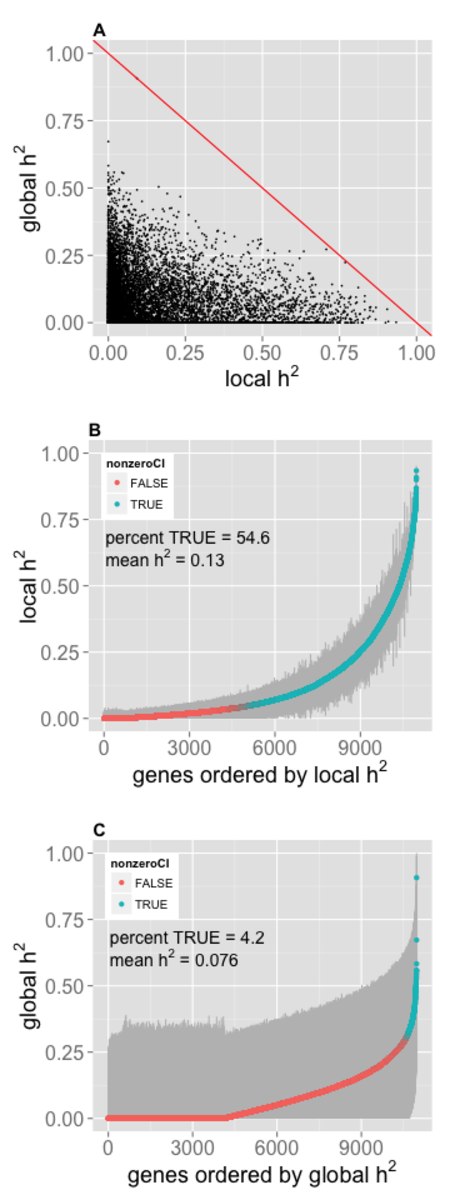
\includegraphics{GenArch_manuscript_files/figure-latex/jointH2-1.pdf}
\caption{DGN-WB joint heritability. Local h\^{}2 is estimated with SNPs
within 1 Mb of each gene. Global h\^{}2 is estimated with SNPs that are
eQTLs in the Framingham Heart Study on other chromosomes (FDR
\textless{} 0.05).}
\end{figure}

\subsection{Citations}\label{citations}

The relationship was first described by Halpern et al. (2006). However,
there are also opinions that the relationship is spurious (Keil \emph{et
al.} 2012). We used R for our calculations (R Core Team 2015), and we
used package \texttt{knitcitations} (Boettiger 2014) to make the
bibliography.

\section{Results and discussion}\label{results-and-discussion}

Lorem ipsum dolor sit amet, est ad doctus eligendi scriptorem. Mel erat
falli ut. Feugiat legendos adipisci vix at, usu at laoreet argumentum
suscipiantur. An eos adhuc aliquip scriptorem, te adhuc dolor
liberavisse sea. Ponderum vivendum te nec, id agam brute disputando mei.

Putant numquam tacimates at eum. Aliquip torquatos ex vis, mei et quando
debitis appareat, impetus accumsan corrumpit in usu. Nam mucius facilis
singulis id, duo ei autem imperdiet instructior. Cu ceteros alienum mel,
id vix putant impedit, ex idque eruditi forensibus eum. Posse dicunt id
usu. Ei iracundia constituto sed, duo ne exerci ignota, an eum unum
conceptam.

Has audire salutandi no, ut eam dicat libris dicunt. Pri hendrerit
quaerendum adversarium ea, dicat atqui munere et sea. Illum insolens eos
ne, eu enim graece rationibus mea. At postea utamur mel, eius nonumes
percipitur at vis. Numquam similique in per, te quo saepe utroque
pericula.

Ea nonumy volumus usu, no mel inermis dissentias. Dico partiendo
vituperatoribus eum et. Mea accusam convenire te, usu populo qualisque
gloriatur ut. Eu eum oratio altera option, ad mea ignota scriptorem. Ne
suas latine vix, eos oblique sanctus pertinax cu.

\section*{References}\label{references}
\addcontentsline{toc}{section}{References}

Boettiger, C. (2014). \emph{knitcitations: Citations for knitr markdown
files}. Retrieved from
\url{http://CRAN.R-project.org/package=knitcitations}

Halpern, B.S., Regan, H.M., Possingham, H.P. \& McCarthy, M.A. (2006).
Accounting for uncertainty in marine reserve design. \emph{Ecol
Letters}, \textbf{9}, 2--11. Retrieved from
\url{http://dx.doi.org/10.1111/j.1461-0248.2005.00827.x}

Keil, P., Belmaker, J., Wilson, A.M., Unitt, P. \& Jetz, W. (2012).
Downscaling of species distribution models: a hierarchical approach (R.
Freckleton, Ed.). \emph{Methods Ecol Evol}, \textbf{4}, 82--94.
Retrieved from \url{http://dx.doi.org/10.1111/j.2041-210x.2012.00264.x}

R Core Team. (2015). \emph{R: A language and environment for statistical
computing}. R Foundation for Statistical Computing, Vienna, Austria.
Retrieved from \url{http://www.R-project.org/}

\end{document}
